\section{Frequency Selective Filters in CT}

Recall the response of stable CT LTI systems to periodic inputs. Given a stable LTI system with frequency response $H(j\omega)$
\[       
x(t) = \sum\limits_{k = -\infty}^{\infty} a_k e^{jk\omega_0 t} \longrightarrow y(t) = \sum\limits_{k = -\infty}^{\infty} a_k H(jk\omega_0) e^{jk\omega_0 t} 
\]

Note the output is equivalent to a signal with Fourier series coefficients $b_k = a_k H(jk\omega_0)$. That is the Fourier coefficients are scaled by the frequency response at the harmonic frequency $k\omega_0$.

Similarly for aperiodic signals, given a stable LTI system with frequency response $H(j\omega)$
\[       
x(t) = \frac{1}{2\pi} \int\limits_{-\infty}^{\infty} X(j\omega) e^{j\omega t}\; d\omega \longrightarrow y(t) = \frac{1}{2\pi} \int\limits_{-\infty}^{\infty} X(j\omega) H(j\omega) e^{j\omega t}\; d\omega 
\]

Note the output is equivalent to a signal with Fourier Transform $Y(j\omega) = X(j\omega) H(jk\omega_0)$. That is the Fourier transform at each continuous frequency $\omega$ is scaled by the frequency response at that frequency.

We can use this behavior to our advantage. In many applications we want to modify the values of $a_k$ selectively, passing them unmodified, increasing (amplifying) them, or decreasing (attenuating) them. This is accomplished by designing a frequency response. Such systems are called frequency selective \emph{filters} and come in 4 basic types:
\begin{itemize}
\item Low-pass Filters attenuate high frequencies while passing through lower frequencies. They are often used to reduce the effects of high-frequency noise in a signal and to prepare it for sampling (so-called anti-aliasing filters). They are the most common filter.
\item High-pass Filters attenuate lower frequencies while passing through higher frequencies. While less common, they are often used to remove the DC component ($\omega$ = 0) of a signal and to compute the derivative of a signal.
\item Bandpass Filters attenuate frequencies outside a band of frequencies. They can be viewed as a combination of a high-pass and low-pass filter. They are commonly used to select a range of frequencies for further processing and are central to many communication technologies.
\item Notch or Bandstop Filters attenuate frequencies inside an often narrow band of frequencies. Common applications are the removal of one or more corrupting signals mixed into another signal.
\end{itemize}

While the design of such filters is outside the scope of this course, you are now equipped to understand and apply them based on your knowledge of the Fourier methods covered over the past several weeks.

\subsection{Ideal Filters}

The above filter types each have an ideal (although unrealizable) form.

Low-pass filters remove frequency content above a threshold, $\omega_c$, called the \emph{cutoff frequency}. They have an ideal frequency response
\[
H(j\omega) = \left\{ \begin{array}{lc}
  1 & -\omega_c < \omega < \omega_c\\
  0 & \text{else}
\end{array}
\right. 
\]
with magnitude and phase plot
\begin{center}
  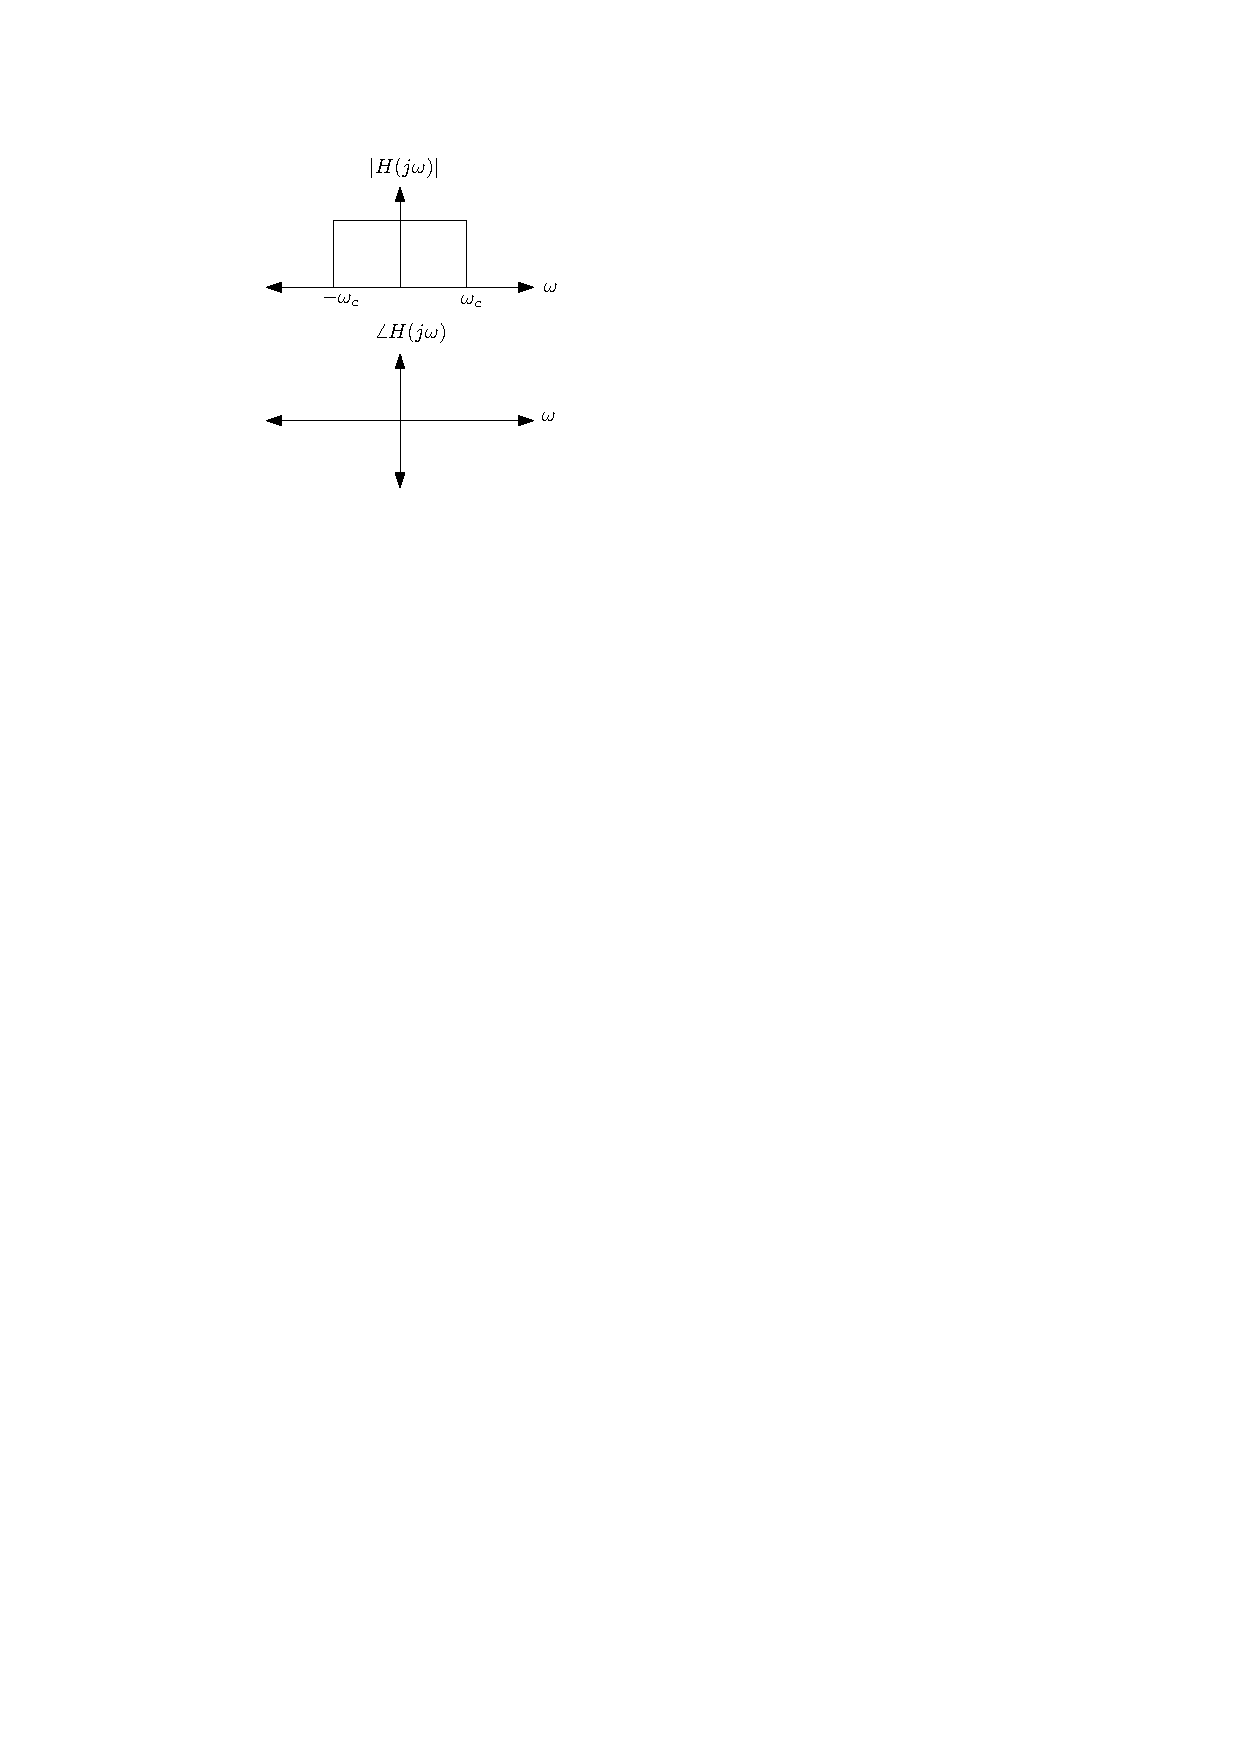
\includegraphics[scale=1]{graphics/lowpass-ideal.pdf}
\end{center}
The range of frequencies below $|\omega_c|$ are called the pass-band. The range of frequencies above $|\omega_c|$ are called the stop-band.

High-pass filters remove frequency content below the cutoff frequency $\omega_c$. They have an ideal frequency response
\[
H(j\omega) = \left\{ \begin{array}{lc}
  0 & -\omega_c < \omega < \omega_c\\
  1 & \text{else}
\end{array}
\right. 
\]
with magnitude and phase plot
\begin{center}
  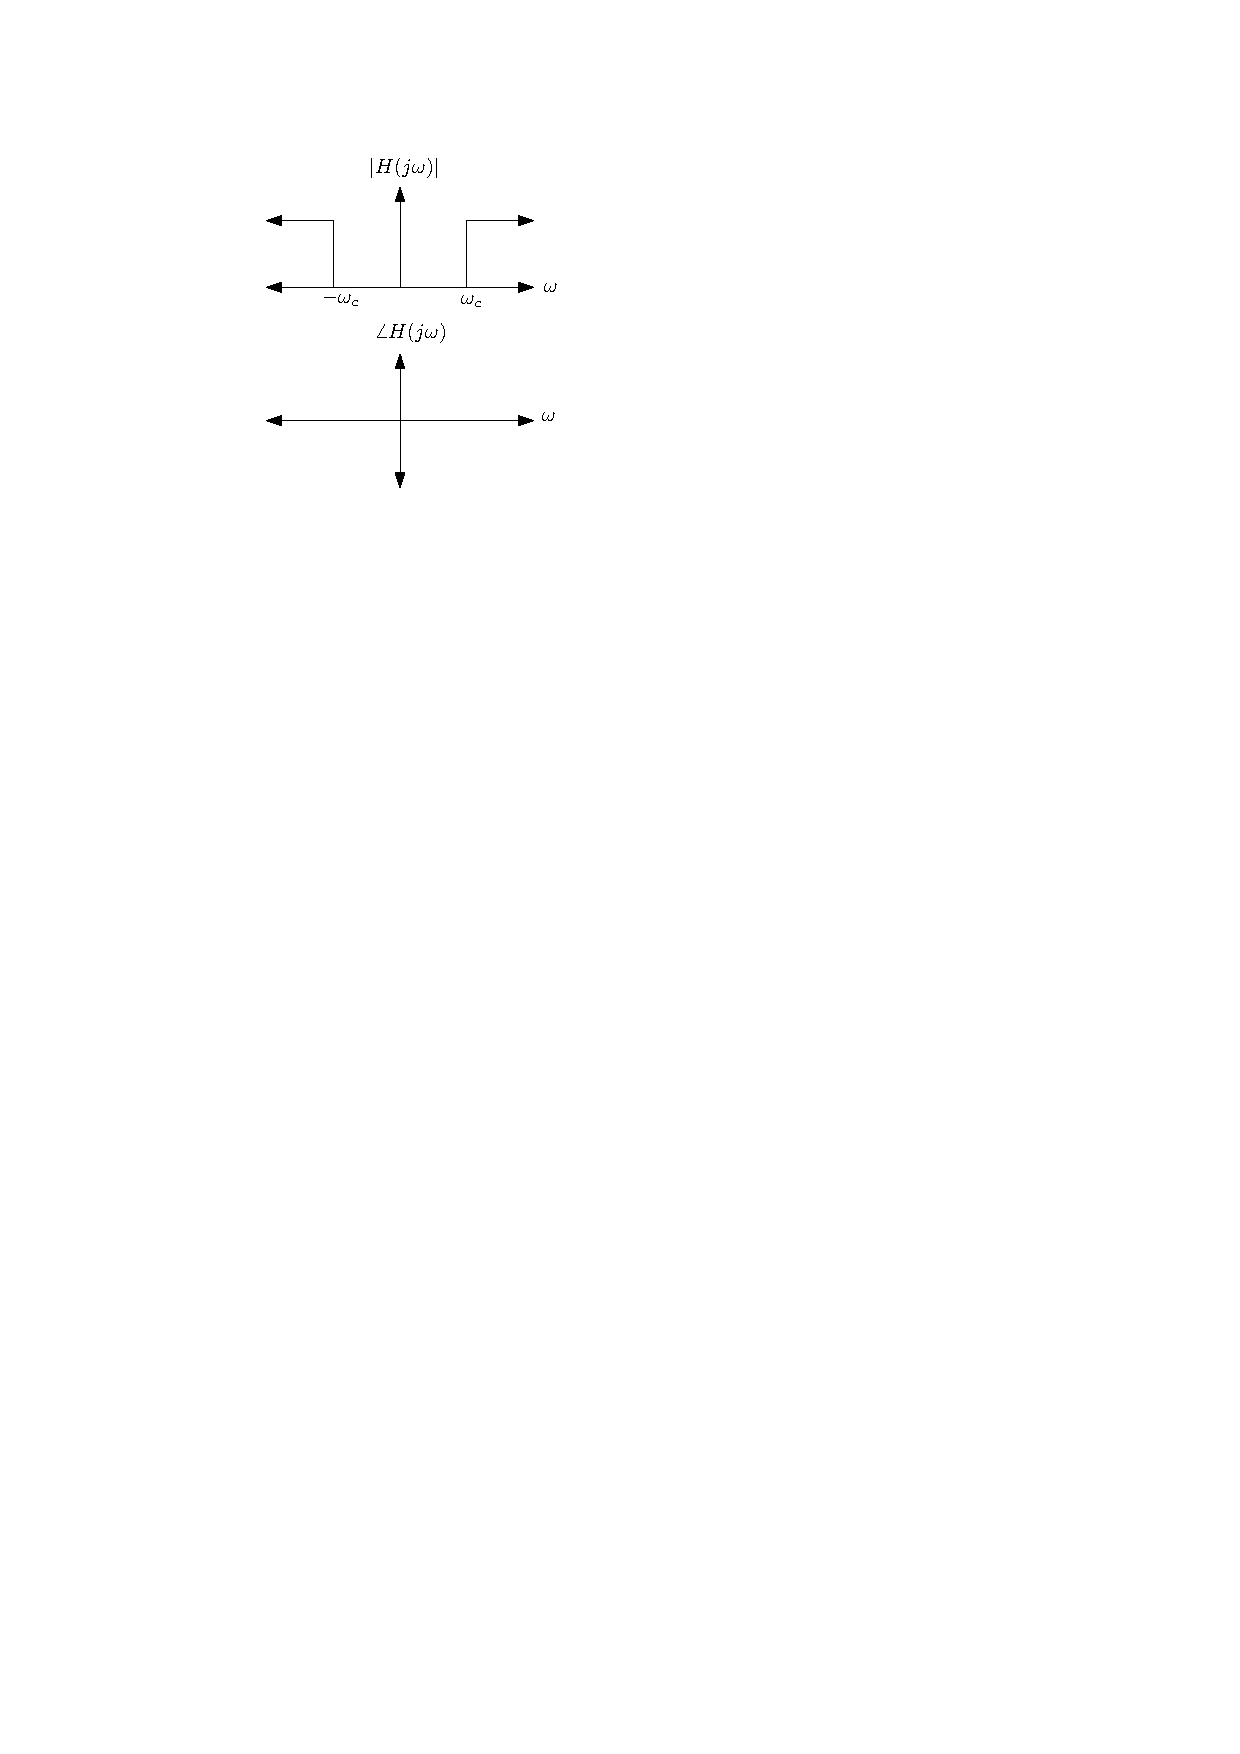
\includegraphics[scale=1]{graphics/highpass-ideal.pdf}
\end{center}
The range of frequencies above $|\omega_c|$ are called the pass-band. The range of frequencies below $|\omega_c|$ are called the stop-band.

Bandpass filters remove frequency content outside a band of frequencies called the pass-band. They have an ideal frequency response
\[
H(j\omega) = \left\{ \begin{array}{lc}
  1 & -\omega_0 - \frac{B}{2} < \omega < -\omega_0+\frac{B}{2}\\[1em]
  1 & \omega_0 -\frac{B}{2} < \omega < \omega_0+\frac{B}{2}\\[1em]
  0 & \text{else}
\end{array}
\right. 
\]
where $\omega_0$ is the \emph{center frequency} and $B$ is the \emph{bandwidth}. The frequencies outside this range are in the stop-band. The magnitude and phase plot looks like
\begin{center}
  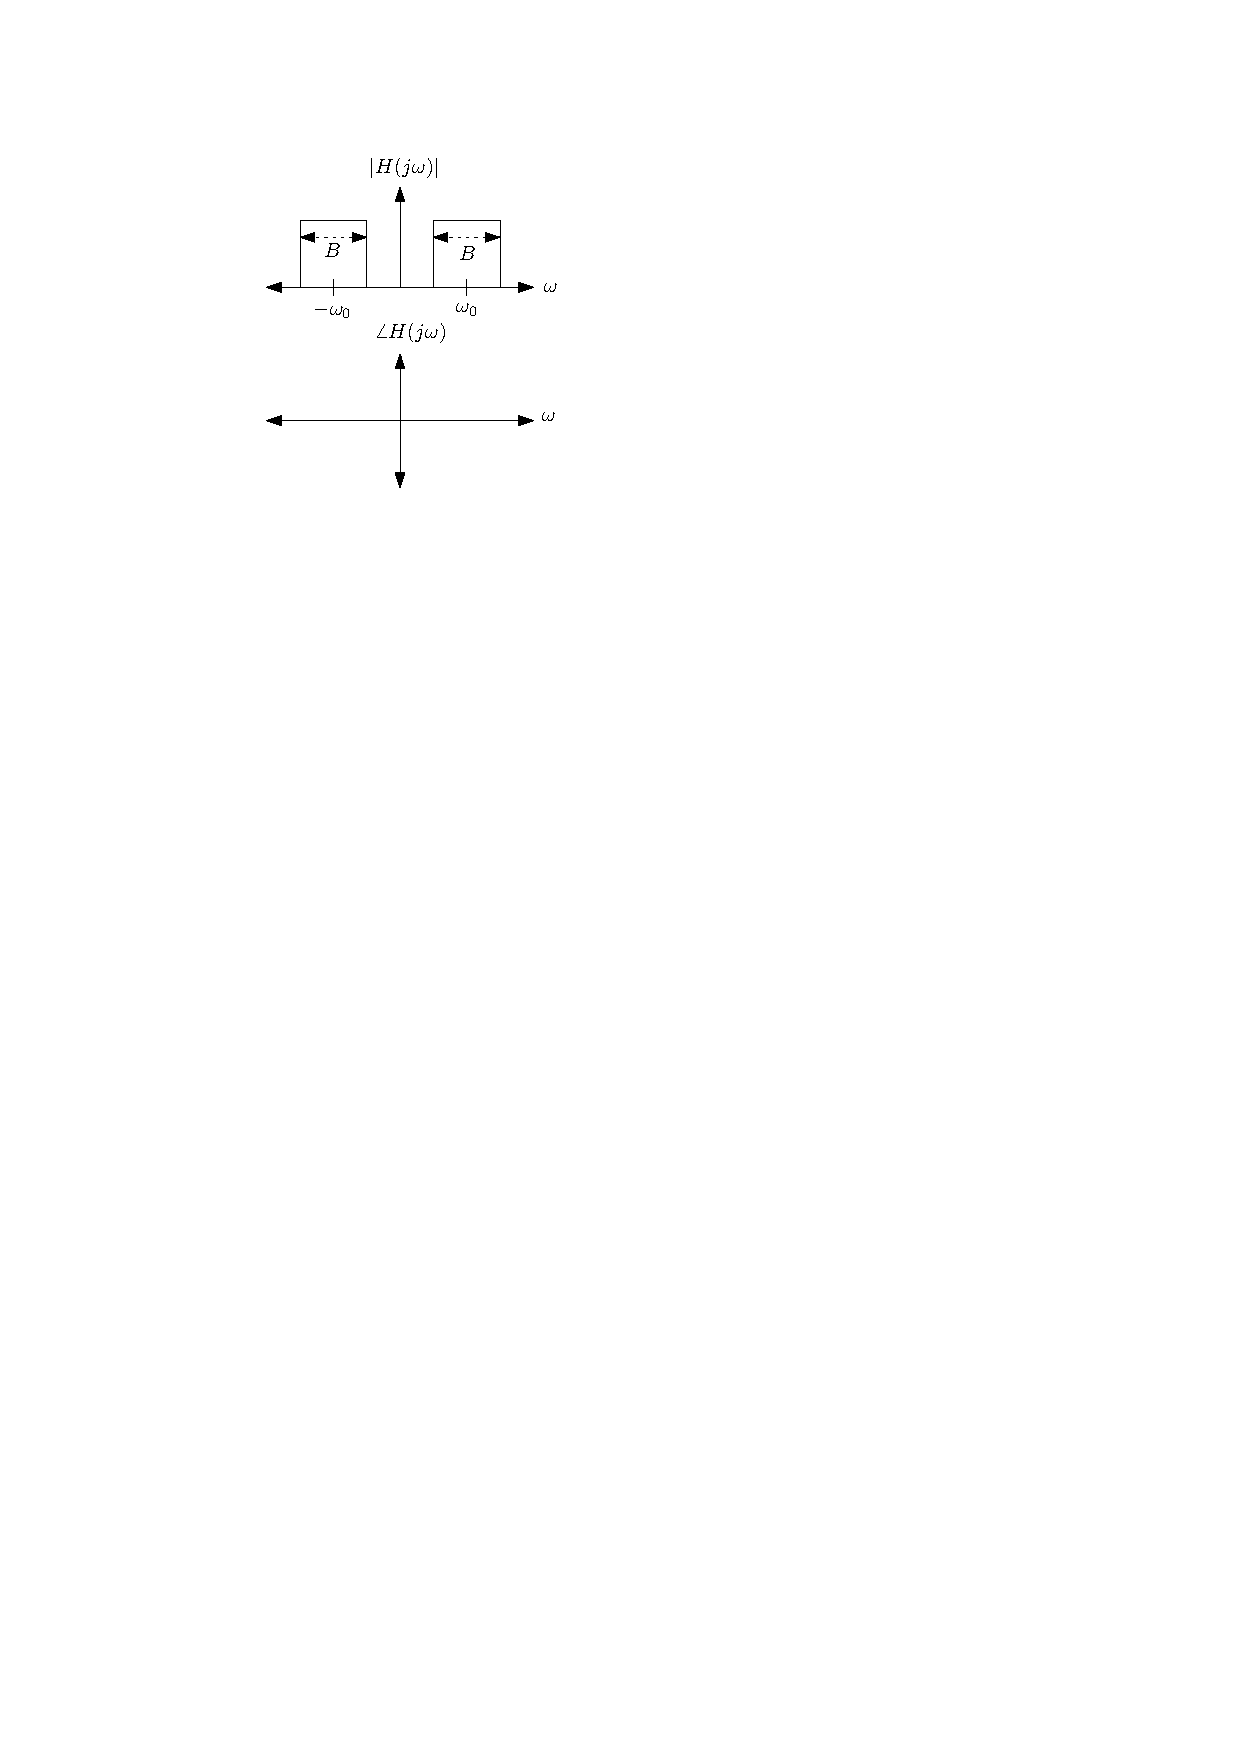
\includegraphics[scale=1]{graphics/bandpass-ideal.pdf}
\end{center}

Finally, notch or bandstop filters remove frequency content inside a band of frequencies (the stop band) defined by the center frequency $\omega_0$ and bandwidth $B$. The ideal frequency response is
\[
H(j\omega) = \left\{ \begin{array}{lc}
  0 & -\omega_0 - \frac{B}{2} < \omega < -\omega_0+\frac{B}{2}\\[1em]
  0 & \omega_0 -\frac{B}{2} < \omega < \omega_0+\frac{B}{2}\\[1em]
  1 & \text{else}
\end{array}
\right. 
\]
with magnitude and phase plot
\begin{center}
  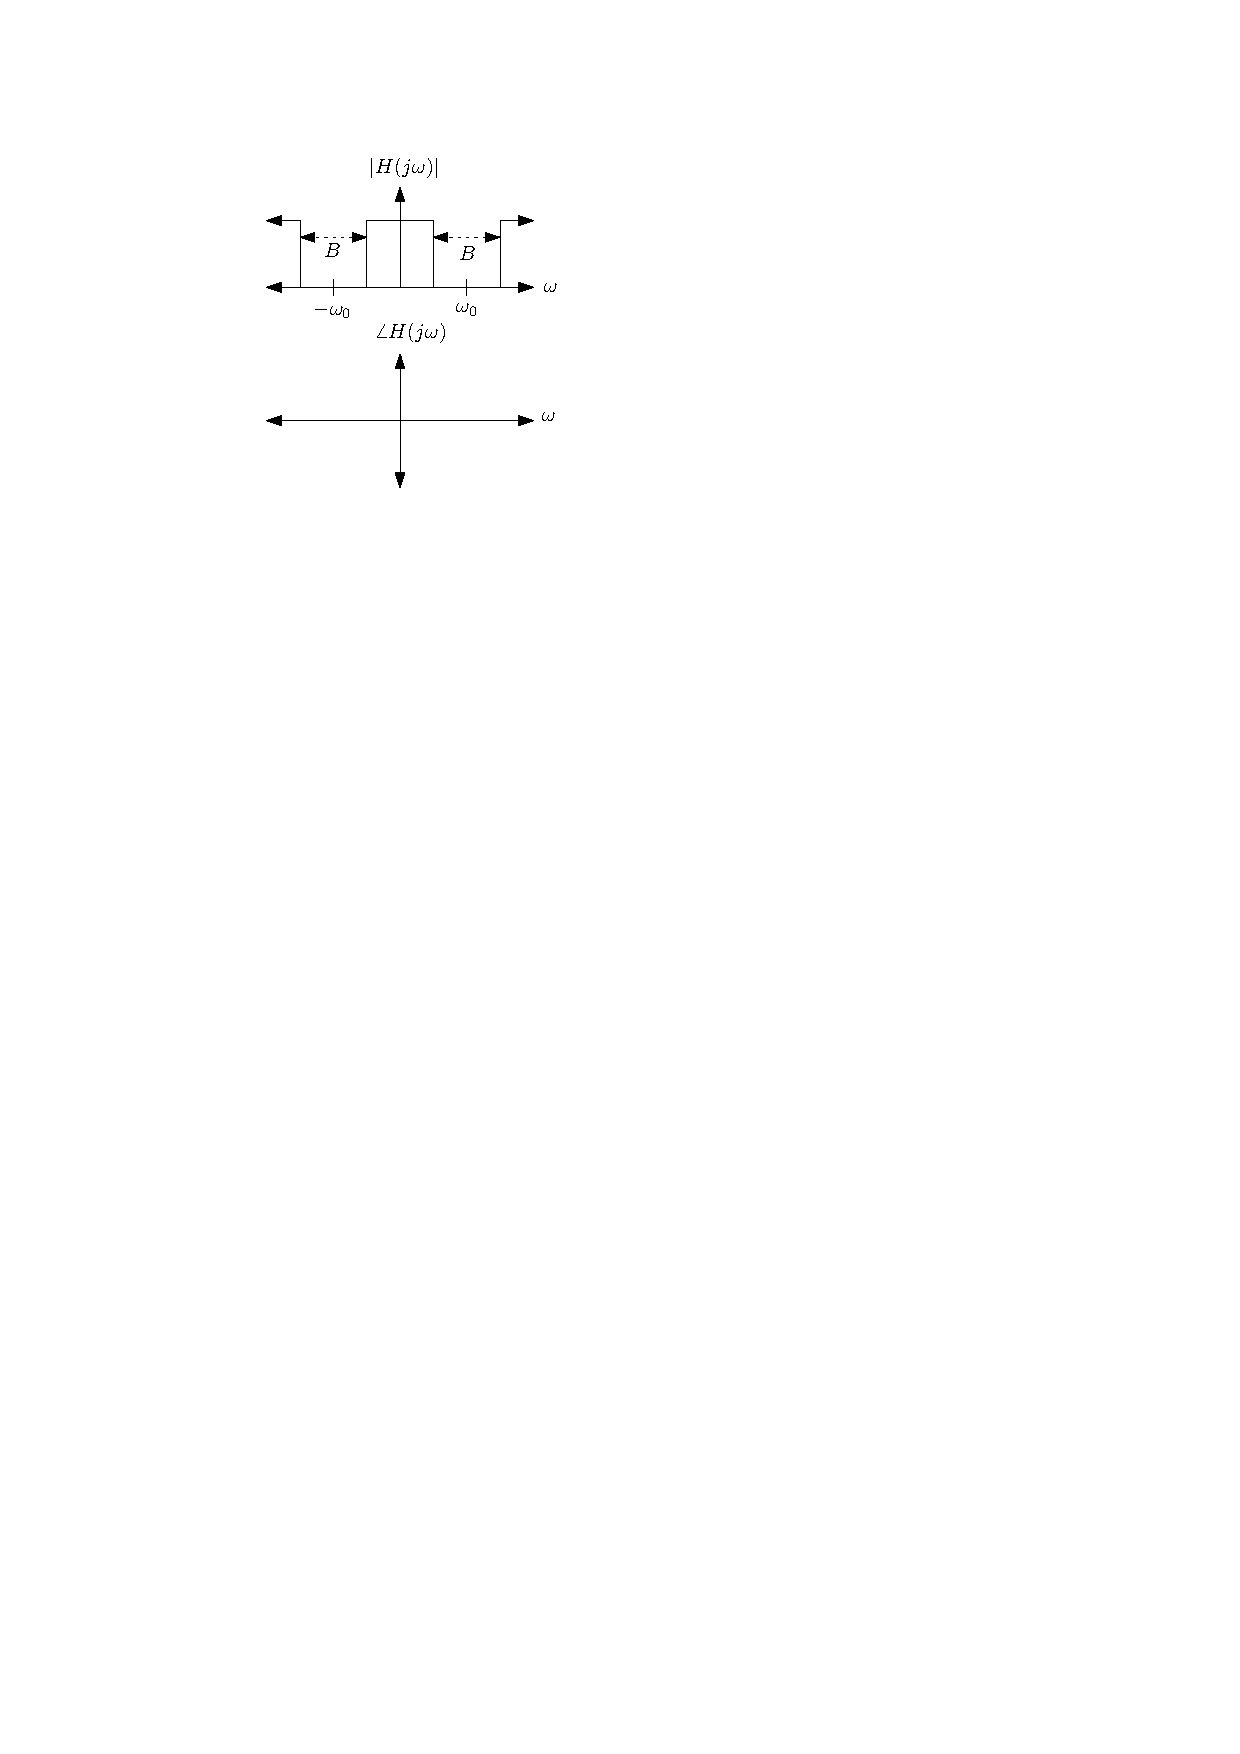
\includegraphics[scale=1]{graphics/bandstop-ideal.pdf}
\end{center}
Often the bandstop filter has a very narrow bandwidth, thus it "notches" out a frequency component of the input signal.

\subsection{Practical Filters}

Ideal CT filters cannot be implemented in practice because they are non-causal and thus physically impossible. To see why consider the impulse response of the ideal low-pass filter:

\[
h(t) = \mathcal{F}^{-1} \left\{ H(j\omega) \right\} = \frac{1}{2\pi} \int\limits_{\-\omega_c}^{\omega_c} e^{j\omega t} \; d\omega = \frac{1}{\pi t}\sin(\omega_c t) 
\]
which has nonzero values for $t < 0$, and thus corresponds to a non-casual system. Ideal filters also have zero phase which cannot be achieved in practice.

Practical filters are described by a frequency response that is a ratio of two polynomials in $j\omega$, i.e.
\[
H(j\omega) = \frac{K \cdot(j\omega - b_1)\cdot(j\omega - b_2)\cdots (j\omega - b_M)}{(j\omega - a_1)\cdot(j\omega - a_2)\cdots (j\omega - a_N)}
\]
where $K$ is a constant that controls the gain at DC, and the zero or more complex coefficients $b_k$ and the one or more complex coefficients $a_k$ are called the \emph{zeros} and \emph{poles} of the filter respectively. Such systems correspond to differential equations as we have covered before and are physically realizable as circuits if all poles and zeros are real or come in conjugate pairs. The processes of designing filters consists of choosing the poles and zeros, or equivalently choosing the coefficients of the numerator and dominator polynomials. This is covered in ECE 3704, ECE 4624, and other upper-level courses. 

Practical filters differ from ideal filters in that they cannot be zero over any finite range of frequencies and cannot transition discontinuously between stop and pass bands. Instead they must vary over the bands and transition smoothly, with a degree of variation and sharpness that is a function of the order of the filter and the exact form of the frequency response polynomials. Thus practical filters are described by additional parameters that define the stop and pass-bands.

The overall gain of the filter is the magnitude of the frequency response at a frequency that depends on the filter type, zero for a low-pass filter and the center frequency for a band-pass filter. The pass-band is defined by the frequency at which the magnitude of the frequency response drops below the overall gain, often -3dB = $\frac{\sqrt{2}}{2}$. The stop-band is defined similarly, as the frequency at which the magnitude of the frequency response drops further below the overall gain, often -20dB = 0.1 or -40dB = 0.01. The \emph{transition bandwidth} is defined as the difference in the stop-band and pass-band frequencies. The \emph{pass-band ripple} is defined as the maximum deviation from the overall gain, over the pass-band.

\subsection{First-order and second-order systems as filters}

Given the equivalence of LTI systems and linear, constant-coefficient differential equations, block diagrams, impulse responses, and frequency responses, filters can be represented in any of these ways.

We have covered extensively first-order and second-order CT systems and seen how they can be represented variously as circuits, differential equations, block diagrams, and as frequency responses. We now see how they can describe simple filters and serve as building blocks for higher-order filters.

\begin{example} Consider a low-pass filter with the desired characteristics of having a pass-band of -3dB at 1kHz, and a stop-band of -20dB at 10kHz. Suppose this is implemented as a first-order "Butterworth" filter, which can be realized by an RC circuit.
\begin{center}
  \begin{circuitikz}[american voltages,scale=0.8, every node/.style={transform shape}]
    \draw
    (5,2.5) node[op amp, yscale=-1] (opamp1) {}
    (0,3) to[R,l=$R$,o-] (opamp1.+)
    (3,0) to[C, l=$C$] (3,3)
    (0,0) to[short,o-o] (7,0)
    (0,3) to[open, v=$x(t)$] (0,0)
    (7.5,2.5) to[open, v=$y(t)$] (7.5,0)
    (opamp1.-) |- (5,1) -| (opamp1.out)
    (opamp1.out) to[short,-o] (7,2.5);
  \end{circuitikz}
\end{center}

  where $R=99.2k\Omega$ and $C=1.6$nF. This is equivalent to the differential equation
  \[
  \frac{dy}{dt}(t) + a y(t) = a x(t)
  \]
  where $a=\frac{1}{RC}$, or the block diagram
  \begin{center}
  \tikzstyle{block} = [draw, fill=gray!20, rectangle, 
    minimum height=2em, minimum width=2em]
  \tikzstyle{sum} = [draw, fill=gray!20, circle, node distance=1cm]
  \tikzstyle{input} = [coordinate]
  \tikzstyle{output} = [coordinate]
  \tikzstyle{pinstyle} = [pin edge={to-,thin,black}]
  
  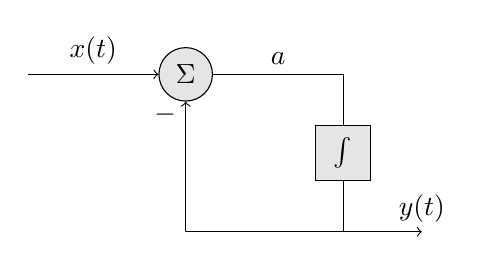
\begin{tikzpicture}[auto]
    \node [input, name=input] at (0,0) {};  	
    \node[block] at (4,-1) (block2) {$\int$};

    \node [shape=coordinate, name=conn] at (4,0) {};
    \node [shape=coordinate, name=conn2] at (2,-2) {};
    \node [shape=coordinate, name=conn3] at (4,-2) {};
    \node [sum, right of=input,node distance=2cm] (sum) {$\Sigma$};
    \node [output, right of=conn3] (output) {};
    
    \draw (sum) -- node {$a$} (conn);
    \draw (conn) -- (block2);
    \draw (block2) -- (conn3);
    \draw (conn3) -- (conn2);
    \draw [->] (conn2) -| node[pos=0.95] {$-$} (sum);
    \draw [draw,->] (input) -- node {$x(t)$} (sum);
    \draw [->] (conn3) -- node[pos=1] {$y(t)$} (output);
  \end{tikzpicture}
  \end{center}
  
  This system has the impulse response
  \[
  h(t) = ae^{-at}u(t)
  \]
  and the frequency response
  \[
  H(j\omega) = \frac{a}{j\omega + a}
  \]
  If we plot the frequency response as a Bode plot, we see the DC gain is 0dB, and the response passes through -3dB and -20dB at the expected frequencies $2\pi*1000 \approx 6.3\times 10^3$ rad/s and $2\pi*10000 \approx 6.3\times 10^4$ rad/s. Thus the transition bandwidth is 9kHz. 
  \begin{center}
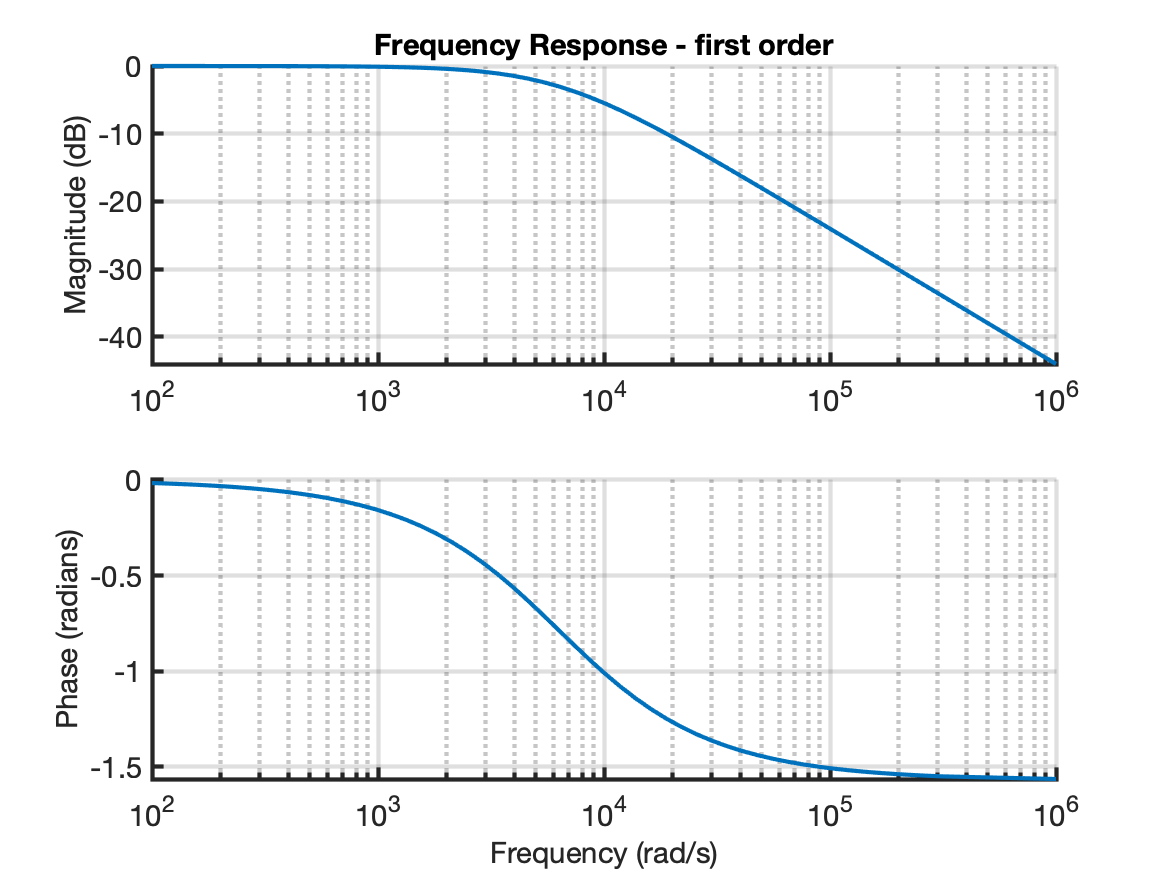
\includegraphics[scale=0.7]{figures/lecture24_1.png}
  \end{center}
  
\end{example}

\begin{example} Suppose we wish to sharpen the transition band for the previous example so that has a pass-band of -3dB at 1kHz, and a narrower stop-band of -20dB at 5kHz. This requires a second-order filter, and can be realized by a circuit called the Sallen-Key.
  
  \begin{center}
    \begin{circuitikz}[american voltages,scale=0.8, every node/.style={transform shape}]
      \draw
      (7,3.5) node[op amp] (opamp1) {}
      (0,4) to[R,l=$R_1$,o-] (2,4)
      (2,4) to[short] (2,5)
      (2,5) to[C,l=$C_1$] (8.2,5)
      (8.2,5) to[short] (opamp1.out) 
      (2,4) to[R, l=$R_2$] (4,4)
      (4,4) to[C, l=$C_2$] (4,0)
      (0,0) to[short,o-o] (12,0)
      (4,4) to[short] (opamp1.-)
      (opamp1.+) to[short] (5.8,1.75)
      (5.8,1.75) to[short] (8.2,1.75)
      (opamp1.out) to[short] (8.2,1.75)
      (opamp1.out) to[short, -o] (12,3.5)
      (0,4) to[open, v=$x(t)$] (0,0)
      (12,3.5) to[open, v=$y(t)$] (12,0);
    \end{circuitikz}
  \end{center}
  where $R_1=74.2k\Omega$, $R_2=91.3M\Omega$, $C_1=1.6$nF and $C_2=160$pF. This is equivalent to the differential equation
  \[
  \frac{d^2y}{dt^2}(t) + 2\alpha \frac{dy}{dt}(t) + \omega_0^2 y(t) = \omega_0^2 x(t)
  \]
  where
  \[
  \alpha = \frac{R_1+R_2}{2R_1 R_2 C_1} \;\text{ and }\; \omega_0^2 = \frac{1}{R_1 R_2 C_1 C_2}
  \]
  or the block diagram
  \begin{center}
    \tikzstyle{block} = [draw, fill=gray!20, rectangle, 
      minimum height=2em, minimum width=2em]
    \tikzstyle{sum} = [draw, fill=gray!20, circle, node distance=1cm]
    \tikzstyle{input} = [coordinate]
    \tikzstyle{output} = [coordinate]
    \tikzstyle{pinstyle} = [pin edge={to-,thin,black}]
    
    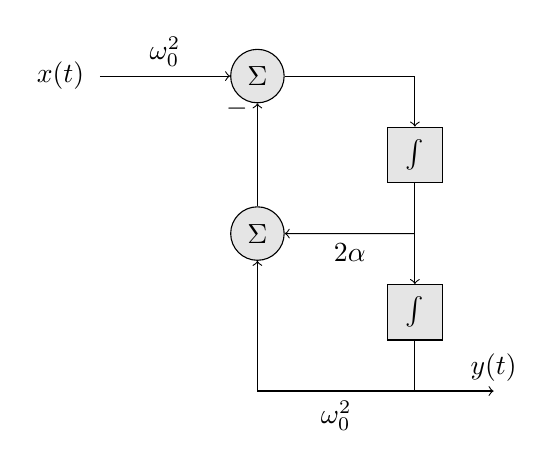
\begin{tikzpicture}[auto]
      \node [input, name=input] at (0,0) {};
      \node [sum, right of=input,node distance=2cm] (sum) {$\Sigma$};
      \node [sum, below of=sum,node distance=2cm] (sum2) {$\Sigma$};
      \node[block] at (4,-1) (block3) {$\int$};
      \node[block] at (4,-3) (block4) {$\int$};
      
      \node [shape=coordinate, name=conn1] at (4,0) {};
      \node [shape=coordinate, name=conn2] at (4,-2) {};
      \node [shape=coordinate, name=conn3] at (4,-4) {};
      \node [shape=coordinate, name=conn4] at (2,-4) {};
      \node [output, right of=conn3] (output) {};

      \draw [->] (input) -- node {$\omega_0^2$} (sum);
      \draw (sum) -- (conn1);
      \draw [->] (conn1) -- (block3);
      \draw (block3) -- (conn2);
      \draw [->] (conn2) -- (block4);
      \draw [->] (conn2) -- node {$2\alpha$} (sum2);
      \draw (block4) -- (conn3);
      \draw (conn3) -- node {$\omega_0^2$} (conn4);
      \draw [->] (conn3) -| (sum2);
      \draw [->] (sum2) -- node[pos=0.95] {$-$} (sum);
      \draw [->] (conn3) -- node[pos=1] {$y(t)$} (output);
      \node at (-0.5,0) {$x(t)$};
    \end{tikzpicture}
  \end{center}
  
  This system has the frequency response
    \[
  H(j\omega) = \frac{\omega_0^2}{\omega_0^2-\omega^2 + j2\alpha\omega}
  \]

  If we plot the frequency response as a Bode plot using the resistor and capacitor values above, we see the DC gain is 0dB, and the response passes through -3dB at the expected frequency $2\pi*1000 \approx 6.3\times 10^3$ rad/s. At the frequency $2\pi*5000 \approx 3.14\times 10^4$ rad/s the response passes through about -28dB. Thus this circuit has a transition bandwidth even narrower than that designed (it is slightly better). 
  \begin{center}
    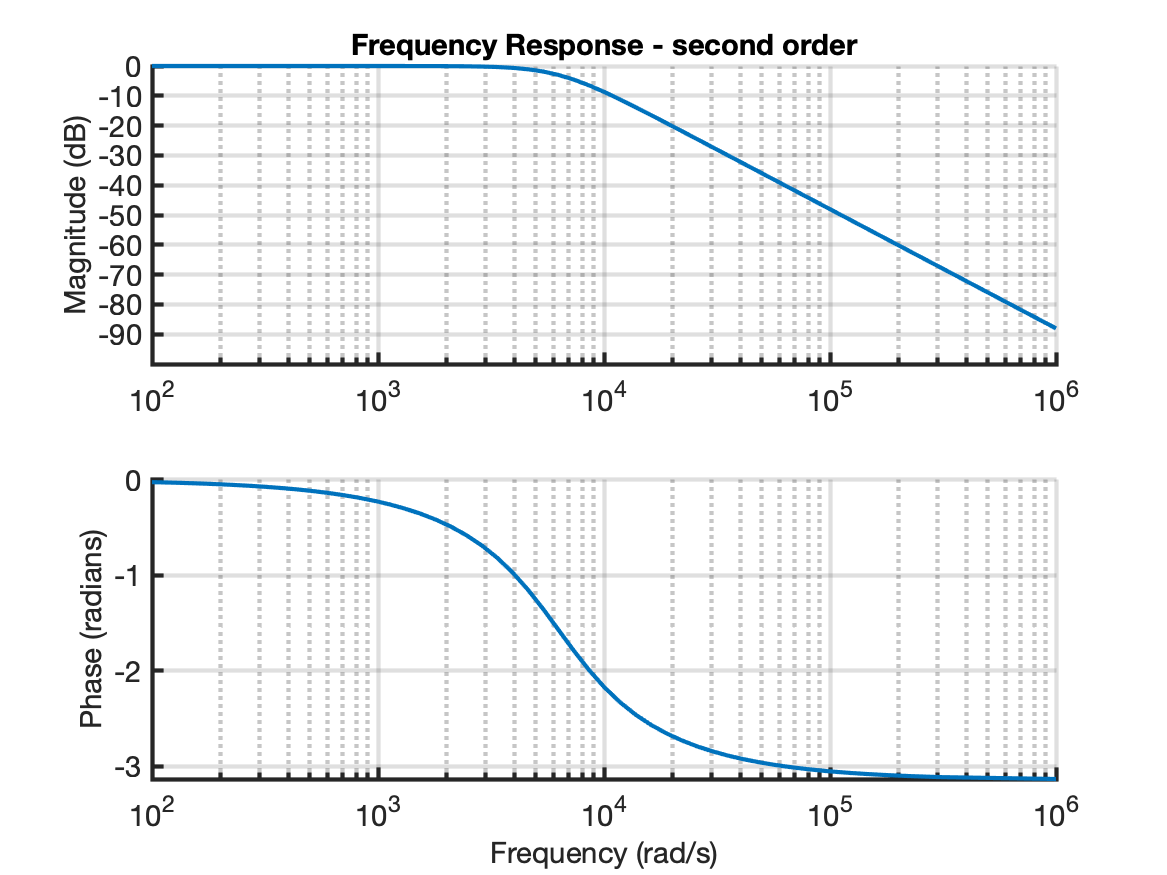
\includegraphics[scale=0.7]{figures/lecture24_2.png}
  \end{center}
  Note the price we pay for this decreased transition bandwidth is a larger phase shift (and a two more components).
\end{example}

\subsection{Higher-Order Filters}

We can continue to increase the steepness of the passband to stop-band transitions by increasing the order of the filter. This is typically accomplished using a serial connection of systems, called \emph{stages} in filter parlance, where each stage is a first-order or second-order system.

Recall in a series connection of systems the overall impulse response is the convolution of the individual responses. If  we assume each stage is stable then, by the convolution property, the overall frequency response is given by the product of their individual frequency responses.
\begin{center}
\begin{tikzpicture}[auto, node distance=2cm,>=latex',scale=1, every node/.style={transform shape}]
    % We start by placing the blocks
    \node [input, name=input] {};
    \node [block, right of=input] (system1) {$H_1(j\omega)$};
    \node [block, right of=system1,node distance=4cm] (system2) {$H_2(j\omega)$};
    \node [output, right of=system2] (output) {};
    \node [right of=output,node distance=1cm] {$Y(j\omega)$};
    \node [left of=input,node distance=1cm] {$X(j\omega)$};
    % Once the nodes are placed, connecting them is easy. 
    \draw [->] (input) -- (system1);
    \draw [->] (system1) -- (system2);
    \draw [->] (system2) -- (output);
\end{tikzpicture}
\end{center}

\[
H(j\omega) = \frac{Y(j\omega)}{X(j\omega)} = H_1(j\omega)\cdot H_2(j\omega)
\]

Writing each response in polar form
\[
H_1(j\omega)\cdot H_2(j\omega) = |H_1(j\omega)|\cdot |H_2(j\omega)| e^{\angle H_1(j\omega)+ \angle H_2(j\omega)}
\]
we note that the magnitudes multiply and the phases add. That means we can use additional stages to reinforce the attenuation of previous stages. Note this requires in the circuit that the stages be impedance isolated, thus the use of the opamps at the end of CT filters. Again the price we pay for increasing the order of the filter and decreasing the transition frequency is increased phase shift in the signal.

\newpage
Matlab code for plotting the first-order example Bode plot:
\begin{verbatim}
R = 99.2e3;
C = 1.6e-9;
a = 1/(R*C);

H = tf([a],[1,a]);
[mag,ph,w] = bode(H);

% Create a nice bode plot 
hFig = figure();
hold on;

subplot(2,1,1);
hm = semilogx(w,20*log10(squeeze(mag)));
grid on;
hTitle  = title ('Frequency Response - first order');
hYLabel1 = ylabel('Magnitude (dB)');
set(gca, 'FontSize', 14, 'YTick', -60:10:20, ...
    'Box', 'off', 'LineWidth', 2);

subplot(2,1,2);
hp = semilogx(w,squeeze(ph*(pi/180)));
grid on;
hYLabel2 = ylabel('Phase (radians)');
hXLabel = xlabel('Frequency (rad/s)');
set(gca, 'FontSize', 14, 'Box', 'off', 'LineWidth', 2);

set(hm, 'linewidth', 2);
set(hp, 'linewidth', 2);
set([hXLabel, hYLabel1, hYLabel2]  , ...
     'FontSize'   , 14          );
set( hTitle                    , ...
     'FontSize'   , 14          , ...
     'FontWeight' , 'bold'      );
\end{verbatim}

\newpage
Matlab code for plotting the second-order example Bode plot:
\begin{verbatim}
R1 = 74.2e3;
R2 = 1.33e6;
C1 = 1.6e-9;
C2 = 160e-12;

a = (R1+R2)/(R1*R2*C1);
b = 1/(R1*R2*C1*C2);

H = tf([b],[1,a,b]);
[mag,ph,w] = bode(H);

% Create a nice bode plot 
hFig = figure();
hold on;

subplot(2,1,1);
hm = semilogx(w,20*log10(squeeze(mag)));
grid on;
hTitle  = title ('Frequency Response - second order');
hYLabel1 = ylabel('Magnitude (dB)');
set(gca, 'FontSize', 14, 'YTick', -90:10:20, ...
    'Box', 'off', 'LineWidth', 2);

subplot(2,1,2);
hp = semilogx(w,squeeze(ph*(pi/180)));
grid on;
hYLabel2 = ylabel('Phase (radians)');
hXLabel = xlabel('Frequency (rad/s)');
set(gca, 'FontSize', 14, 'Box', 'off', 'LineWidth', 2);

set(hm, 'linewidth', 2);
set(hp, 'linewidth', 2);

set([hXLabel, hYLabel1, hYLabel2]  , ...
     'FontSize'   , 14          );
set( hTitle                    , ...
     'FontSize'   , 14          , ...
     'FontWeight' , 'bold'      );
\end{verbatim}
